\documentclass{standalone}

\usepackage{tikz}
\usepackage{url}
\usepackage{xcolor}
\usetikzlibrary{shapes,positioning,matrix}

\definecolor{lightblue}{HTML}{D4EDF7}
\definecolor{blue}{HTML}{7ab9d1}
\definecolor{darkblue}{HTML}{83aedd}
\definecolor{lightorange}{HTML}{FFA364}
\definecolor{orange}{HTML}{FF6802}
\definecolor{darkorange}{HTML}{9C3F00}

\pgfdeclarelayer{background}
\pgfsetlayers{background,main}

\renewcommand{\familydefault}{\sfdefault}
\begin{document}
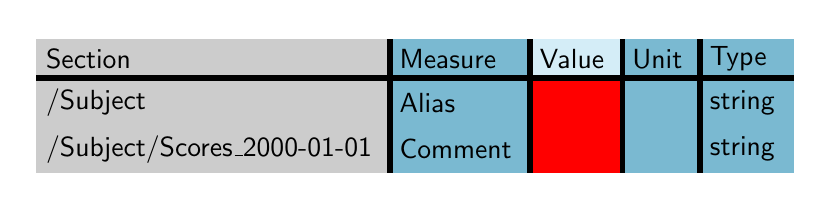
\begin{tikzpicture}[]


\matrix(dict)[matrix of nodes, nodes={align=left, anchor=west, black}]{
    
      Section & Measure & Value & Unit & Type \\
      /Subject & Alias & & & string \\
      /Subject/Scores\_2000-01-01 & Comment & & & string \\
      %/Subject/Scores\_2000-01-02 & Comment & & & string \\
    };

\coordinate (tl) at (dict-1-1.north west);
\coordinate (br) at (dict-3-1.south -| dict-2-5.east);
    
% horizontal line
\draw[line width=2](tl |- dict-1-1.south west)--(br |- dict-1-1.south west);
% vertical lines
\draw[line width=2](tl -| dict-1-2.north west)--(br -| dict-1-2.north west);
\draw[line width=2](tl -| dict-1-3.north west)--(br -| dict-1-3.north west);
\draw[line width=2](tl -| dict-1-4.north west)--(br -| dict-1-4.north west);
\draw[line width=2](tl -| dict-1-5.north west)--(br -| dict-1-5.north west);

\begin{pgfonlayer}{background}
    \path[fill=gray!40]	(tl) rectangle (br -| dict-1-2.west);
    \path[fill=blue]		(tl -| dict-1-2.west) rectangle (br -| dict-1-3.west);
    \path[fill=lightblue]	(tl -| dict-1-3.west) rectangle (br -| dict-1-4.west);
    \path[fill=blue]	(tl -| dict-1-4.west) rectangle (br);
    % highlight empty values
    \path[fill=red] (dict-1-3.south west) rectangle (dict-1-3.south east |- br);
\end{pgfonlayer}




\end{tikzpicture}

\end{document}	

